\chapter{CMS Detector}
\label{CMS_chapter}

In this analysis we are going to perform simulations of collisions occurring at the CMS experiment, so we have to take into account the specific characteristics of this detector. For this reason,
the components of the CMS are going to be explained.
The CMS is one of the seven experiments located at the Large Hadron Collider (LHC), which is the largest and most powerful particle accelerator in the world. This accelerator collides protons 
and heavy ions at very high energies of the order of 13 TeV and 6.37 TeV, respectively, with the objective of studying the elemental particles of the universe. 

%Energia ions http://accelconf.web.cern.ch/accelconf/ipac2016/papers/tupmw027.pdf

The LHC is conformed by a ring of almost 27 km of perimeter and by 7 detectors located at the different collision points of the ring. Two of these detector are general-purpose detectors, and they 
are called experiments CMS and ATLAS. Both experiments share the same goals of searching physics beyond the SM. The physics program of these experiments includes measurements of the Higgs boson, 
Supersymmetry searches, dark matter, detection of extra dimensions, among others. The difference between both experiments is that they use different designs and software. In the ATLAS detector, the 
magnetic field is produced by a central toroid, two end toroids, and a central solenoid, while the CMS detector is built around a superconducting solenoid magnet.  

The CMS and ATLAS detectors have a cylindrical form in order to have the most uniform magnetic field posible. They are centered in the direction of the interacting beams and the collision point and have two ``end-caps'' to cover the forward regions. These detectors are conformed by the same general components, from the inner part of the detector to the outer part. These components are: a tracking system, an electromagnetic and a hadronic calorimeter, and muon detectors. They also have magnets to curve the path of the electric charged particles, so it can be determined whether a particle has a positive or negative charge. Aditionally, the measurement of the curve can be used to calculate the momentum of the charged particle. In Figure \ref{CMS_detector}, there is a diagram showing the structure of the CMS detector. This image also shows the interaction of different particles with the parts of the detector.

%\section{Accelarator and Storage Ring}
%citada imagen http://cms.web.cern.ch/news/detector-overview

 \begin{figure}[h]
 \centering
 \caption{CMS detector. Image take from \cite{CMS_detector_slice}}
 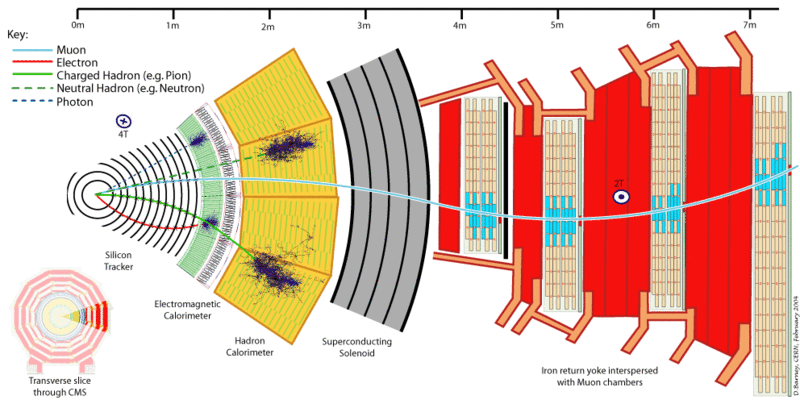
\includegraphics[width=0.9\textwidth]{./Capitulos/CMS/CMS}  
 \label{CMS_detector}
 \end{figure}

\section{Tracking System}

Since every 25 ns there is a collision at the center of the CMS detector and almost 1000 particles are going to be produced, it is necessary to have a tracking system able to record measurements 
of all the particles that are produced. This tracking system must be located the nearest possible to the region where the collision occurs. This tracking system is used to measure the momentum and 
vertices of the particles with a high precision. The inner detectors are built with silicon detectors, with high granularity pixel systems at the smallest radii, and silicon-strip detectors at larger ones \cite{Perspectives_LHC}.

The properties of the tracking system are: fast recording of measurements, tolerance to high radiation doses, ensembled with light material and tolerance of the severe conditions imposed by the low temperature at LHC (of almost 2 K). One of the major challenges for the inner dectector parts is the control of aging effects because the damage produced by irradiation is severe. The silicon detectors are p-n junction diodes, so when a particle crosses the detector, it causes the liberation of electron-hole pairs, which move to the electrodes of the system. The tracking system in the CMS detector covers the range within $|\eta|<2.5$, the region where most of the relevant particles for the analysis arrive. 

The flux of particles arriving to a point in the detector depends on the distance from the center of collision to where the detector is located: as the flux crosses the detector material the quantity of particles decreases. Thus, the resolution of the tracking system does not need to be so high in the intermediate and end caps regions. For this reason, in the first region of the tracking system (the closest to the interaction point), there are silicon pixel detectors with cell size of $100 \times 150 \mu \text{m}^2$. The innermost layer of pixels is located as near to the beam as it is practical, this is at a radius around 4.5 cm.
 
The silicon pixels are expensive and have high power density. Aditionally, the flux of particles at an intermediate region of the inner detectors is low enough to use silicon microstrips. Thus, in the region of radius greater that 20-55 cm, the silicon pixels are replaced by silicon microstrips. These silicon microstrip are arranged in a special way to improve the resolution in the z axis. These barrel cylinders and end-caps disks, as the silicon pixels, cover the region of $|\eta| < 2.5$. The strip dimensions are around $11 \text{cm} \times 100 \mu \text{m}$.

In the outermost region of the tracking system (at a radius greater that 55 cm) the particle flux is low enough to use larger-pitch silicon microstrips. The maximum size of these cells is $25\text{cm} \times 80 \mu \text{m}$. There are 6 layers of these silicon microstrips modules in the barrel and 9 end-caps disks that also cover the region given by $|\eta|< 2.5$.

%Escribir interaccion particulas con tracking systems

\section{Calorimetry}

Surrounding the tracking system of the CMS detector are located the electromagnetic and hadronic calorimeters. The calorimeters measure the energy of the incoming particles by absorbing the particles and transforming them into heat. The priorities of the electromagnetic calorimeter are to measure precisely the energy of electrons and photons, and to make measurements of their position and direction of movement. The priorities of the hadronic calorimeter are to make precise measurements of the jets energy and to cover a larger area of $|\eta| < 5$. The area covered has to be large with the purpose of attributing all the $\vec{E}_T^{miss}$ to the particles that cannot be detected \cite{Perspectives_LHC}. 

The electromagnetic and hadron calorimeters are made out of scintillation crystals. When a high energy particle goes through the detector, it collides with the nuclei of the material and generates a shower of particles. The product particles of this interaction excite the atoms in the material by making the electrons in the material go to a higher orbit. When each electron returns to the initial orbit, it emits a photon. 

Then, the light emmited by the scintillator is measured by photodiodes, which have the function of converting the optical signals into electronic signals. The photodiodes mechanism is based on the photoelectric effect: the photons emitted by the scintillator arrive to the light-sensitive area of the photodiode and expulse electrons in this surface. Then, these electrons are accelerated and strike a silicon diode target, which causes that more electrons get expelled of this surface. At the end, one obtains an amplification of the initial signal which is measured.

\subsection{Electromagnetic Calorimeter}

The electromagnetic calorimeter is an entirely active homogeneus calorimeter made of lead tungstate (PbWO$_4$) crystal. It has 61,200 crystal in the central barrel part and 7,324  in each of the two end-caps. As a consequence from the use of high density crystals, the calorimeter is fast, has fine granularity and is radiation resistant. 

The lead tungstate crystal material was chosen for different reasons. First, it emits a short radiation length which is easy to record. Second, it has small Moliere radius, which is defined as the radius of the cylinder surrouding the 90\% of the shower's energy deposition. That leads to a compact calorimeter in size. Third, the lead tungstate crystal has short decay time constant, which allows the calorimeter to have a fast response. Lastly, it is resistant to high doses of radiation. Moreover, due to the electromagnetic calorimeter is located within the solenoid, avalanche photodiodes are used as photodetector because they can operate under the magnetic field of 4T \cite{Perspectives_LHC}. 

\subsection{Hadron Calorimeter}

Surrouding the electromagnetic calorimeter is located the hadron calorimeter. Its objective is to measure the energy and direction of jets. It is designed to detect the most possible particles product of a collision, so it is said that the detector has a hermetic coverage. The priority of this calorimeter is to determine as correct as possible the missing transverse energy ($\vec{E_T^{miss}}$). The hadron calorimeter is made out of plastic scintillator tiles with wavelenght-shifting fiber. The wavelength-shifting is used to shift the wavelenght of the light emitted by the scintillator in a the range in which the efficiency of the photodiodes is high \cite{Perspectives_LHC}.

The hadron calorimeter is restricted to fill the area between the outer cap of the electronic calorimeter and the magnet coil, this is $1.77 \text{m} < R < 2.95\text{m}$. The layers of the scintillator tiles are alternately placed with layers of copper in the barrel to form the hadron calorimeter. The end-caps of the calorimeter covers the area of pseudorapidity given by $|\eta|= 3$ and $|\eta|= 5$.


\section{Muon Detector}

The muon system detector consists of several multi-layer large area gas-based detectors. The main objective of this detector is to take precise measurements of muon tracks. Since the muon system 
detector is located at the outermost part of the CMS, the radiation level it receives is very low in comparison to the tracking system and the calorimeters. The CMS muon detector has three tasks: 
to identify the muon particles, measure its momentum and triggering on them (this concept is explained in the next subchapter). The layers of the muon detector alternate with layers of the yoke where 
the magnetic field returns, which is called flux-return yoke \cite{Perspectives_LHC}. 

The flux-return yoke curves the path of the particles in the opposite direction as it was inside the copper layers. It also can be used for good resolution muon identification because it absorbs 
some hadrons with low energy. The high magnetic field applied and the flux-return yoke allows to take precise measurements of the muon momentum. The muon system detector surrounds the hadron
calorimeter and consists also of a barrel section and two end-caps. 

The CMS detector has three types of gaseous particle detectors for muon measurements. In the barrel region where the neutron-induced background is low and the magnetic field is almost uniform, 
there are located drift chambers. The drift chambers are tubes each of 4 cm wide that contain a strechted wire immersed in a gas. When a muon crosses the chamber, it hits the electrons of the atoms
in the gas. Then, the free electrons arrive to the positive charged wire and an electronic signal is measured. By measuring the time it takes for an electron to arrive to the cathode (known as 
drift-time) and the velocity of the free electrons (drift velocity), it is possible to determine the position of the initial muon \cite{Muon_drift_tubes_cms, Particle_Detectors_Claus}. The drift chambers cover the region of pseudorapidity given by 
$\eta < 1.2$.
%Referenciaaaaaaaaaaa: http://cms.web.cern.ch/news/muon-drift-tubes
%REferenciaaaaaaaaaaaa: Claus gruppen - Particle detectors 
  
In the two-end caps regions there are cathode strip chambers (CSC). In these regions the muon rates and backgrounds levels are high and the magnetic field is large and non-uniform. The CSC uses the
same principle as the drift chamber to measure the position of muons. The difference is that the CSC consist of anode wires crossed with cathode strips, and these arrays are also immersed in a gas. When
a charge particle crosses the detector, it hits the atoms of the gas expelling electrons. The free electrons are guided by the electric field and arrive to the anode wires, while the positive ions 
move towards the cathode \cite{CSC_CMS}. The CSC have fast response time, fine segmentation and are radiation resistant. Thus, they are able to take precise measurements of time and position. These detectors cover the
area given by $|\eta| < 2.4$. Due to the fact that the tracking system and muon detectors take indepedent measurements of the muon momentum, it is possible to find errors and check both measurements 
\cite{Perspectives_LHC}.

%http://cms.web.cern.ch/news/cathode-strip-chambers

An additional redundacy in the muon measurements is contributed by resistive plate chambers (RPC) in the barrel and the two end-caps regions. It is similar to the other two muons detectors: it is 
conformed by two plates, one is the cathode and the other the anode and these plates are separated by a gas. When a charged particle crosses the detector, the resulting free electrons move to the anode.
The electric signal is received by metallic strips after a precise time delay \cite{RPC_CMS}. The set of hit strips gives a precise measurement of the muon position and momentum.
%http://cms.web.cern.ch/news/resistive-plate-chambers

\section{Triggers}

Since at the LHC there are bunch crossings every by 25 ns with a peak crossing rate of 31.6 MHz, nearly a billion proton-proton events are produced every second. Thus, it is necessary to decide
to store or not store an event in order to reduce the computational resources use. Triggers have the task of applying a primary selection on the data at real-time. The triggers take the data and quickly 
decide which events that are interesting pass to the next phase of filtering. The triggers need to have a rejection factor of almost $10^7$. As a consequence, it allows to store just around 100-200 
carefully selected events per second to be proccessed later. 

The first triggering level uses a partial amount of the total information given by the detector and takes decisions in less that 3.2 ns. 
It reduces the data rate to nearly 100 kHz \cite{LHC_collitions_web}. High level triggers use a network of thousands of processors and fast switches. They get the information gradually and use algorithms in order to reduce 
the amount of data. The final product is that at a rate of 150-200 Hz each event occupies around 1.5 Mb. The former leads to the LHC to have an annual data volume of around 10 PB \cite{Perspectives_LHC}. After an event 
passes the first triggering level, the resulting data is transferred from the detector electronics into readout buffers. Then, the signal is processed and compressed while the events are studied by 
processors with several thousands of central processing units. The event then is directed to a single processor with the objective of performing detailed calculations of the critical parameters of the 
event and reduce the amount of data.

%https://lhc-machine-outreach.web.cern.ch/lhc-machine-outreach/collisions.htm





